\chapter{The Hardware Architecture of a High-Speed Router}
\label{chap:arch}
%TODO: We should say what we mean by shared memory later? It's confusing to
%dismiss shared-memory here and then talk about shared memory routers later.
%Really the shared-memory in shared memory routers refers to the scheduler and
%(to a lesser extent) the sharing of the pipeline across the ports of the
%routers.

This chapter describes the hardware architecture of a high-speed router to
provide a mental model of a router chip for the rest of this dissertation. We
first describe the main functions of a router. We then describe the performance
requirements for a high-speed router today. Motivated by these performance
requirements, we consider two strawman hardware architectures and explain why
they fall short. We then describe the predominant pipeline-based architecture
of high-speed routers today.

\section{Overview of a router's functionality}

A router's functionality can be divided into two major planes: the {\em control
plane} and the {\em data plane}. The control plane is responsible for running
distributed routing protocols (\eg BGP, IS-IS, and OSPF), creating access
control rules, and setting up tunnels for network virtualization. The control
plane populates a router's {\em match-action tables}:\footnote{Also known as
lookup tables, routing tables, or just tables.} tables that carry out a
specific action on a packet if the packet matches a particular pattern in an
incoming packet. As an example, a match-action table could instruct the router
to transmit a packet on a particular port (action) if the packet has a certain
destination address (match). The data plane is responsible for carrying out the
match-action operation on each packet. It matches the relevant packet headers
against the match part of a match-action table entry and performs the
appropriate action on the packet's headers.

The control plane typically runs when the network's topology changes or when a
network's policy changes. The data plane, on the other hand, needs to run on
every packet. The rate of policy or topology changes is typically much lesser
than the rate at which packets are processed at a router. Hence, the control
plane runs on a general-purpose CPU, while the data plane is implemented in a
dedicated hardware as part of a router chip or ASIC.
Figure~\ref{fig:router_box} shows an example router with its control and data
plane.

\begin{figure}
\centering
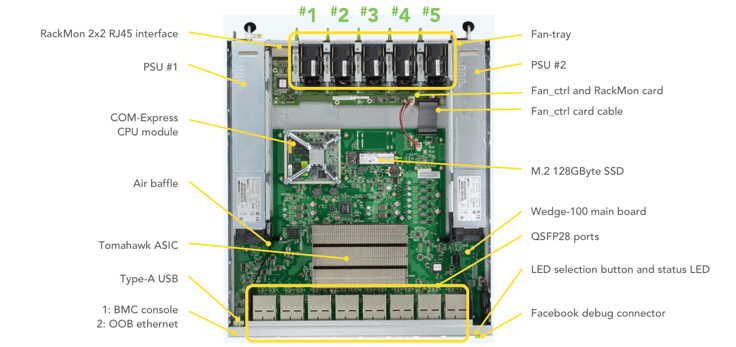
\includegraphics[width=\textwidth]{wedge100.png}
\caption{Facebook's Wedge 100 router from the Open Compute Project~\cite{ocp}.
The COM-Express CPU module serves as the control plane, while the Tomahawk ASIC
is a router chip that serves as the data plane. Image courtesy of
Facebook~\cite{wedge100}.}
\label{fig:router_box}
\end{figure}

\section{Performance requirements for a high-speed router}
Because this dissertation focuses on programmability of router features that
were historically implemented in fixed-function hardware, we focus on the
architecture of the data plane here. To motivate a hardware design for the
router chip, it is useful to have a sense of the performance requirements of a
high-speed router. For illustration, let's consider a high-speed 1 Tbit/s
router, representative of many high-speed routers today~\cite{trident2,
tomahawk, tomahawk2}. Let's assume that the router needs to forward 1000 bit
packets. Finally, let's assume that on each packet, the router needs to carry
out \textasciitilde10 operations, such as determining the output port based on
the destination address, access control, tuneling, measurement, and
decrementing the IP TTL field. These requirements translate into the need to
support about 10 operations on a billion packets per second, or equivalently, 10
billion operations per second.

\section{Strawman 1: a single 10 GHz processor}
One approach to architecting a router chip is to build a single in-order scalar
processor that can run at 10 GHz and support 10 billion packet operations per
second (Figure~\ref{fig:single_processor}). But these clock rates are out of
reach today; even with painstaking manual design, the fastest general purpose
processor chips today do not exceed 10 Ghz, and most other chips (\eg graphics
processors and digital signal processors) have lower clock speeds in the 1 GHz
range.

\section{Strawman 2: an array of processors with shared memory}

An obvious solution to this problem is to have many scalar in-order processors
operate in parallel on different packets. When a packet comes in, a distributor
could send a packet to a free in-order processor, which would then carry out
all the operations on that packet, before accepting a new packet. This
architecture is similar to some network processors~\cite{ixp1200, ixp2800,
quantumflow}.  These network processors featured an array of simple processors,
and each of these processors would handle all the operations corresponding to a
single packet.  With such an approach, to handle 10 billion operations per
second, we would need 10 processors. Each processor would perform 1 billion
operations per second, which is much more feasible
(Figure~\ref{fig:processor_array}).

%TODO: Try and clean up paragraph below.
The problem with this approach is that the match-action tables need to be
shared across all processors, to allow any processor to match packets against a
match-action table on every clock cycle. In effect, the memory housing the
match-action table needs to support 10 billion matches (reads) per second even
though the actions corresponding to these matches can be performed
independently on each packet by each processor. Memory designs typically run at
the same clock frequency as the processor (1 GHz) and support a single read or
write operation per cycle (also known as single-ported memory). Supporting 10
billion matches per second requires a {\em multi-ported} memory capable of
handling multiple read operations every clock cycle (where a clock cycle is 1
ns). Such multi-ported memory modules consume considerably more area than
standard single-ported memory.

\begin{figure}[!t]
\begin{minipage}{0.3\textwidth}
\centering
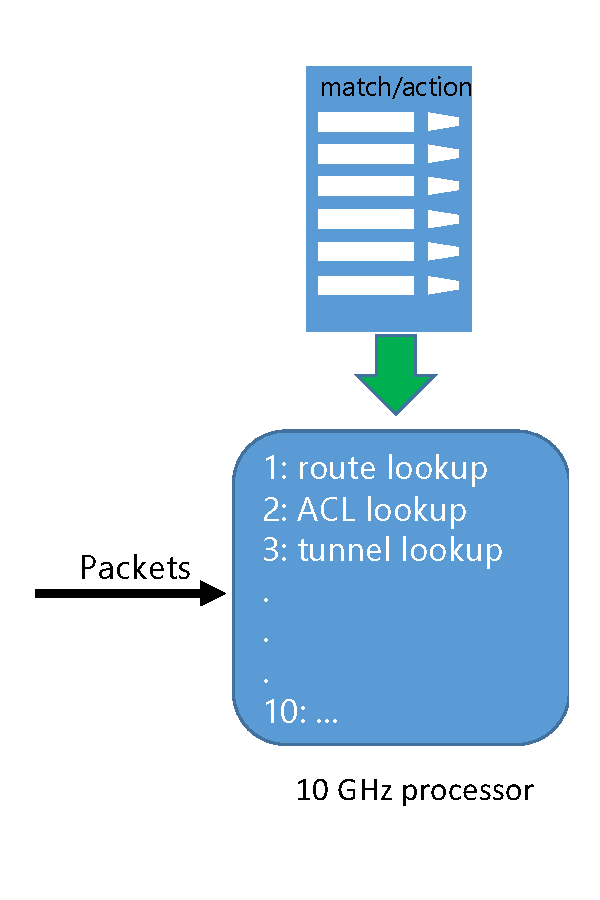
\includegraphics[width=\textwidth]{single_processor.pdf}
\caption{10 GHz processor}
\label{fig:single_processor}
\end{minipage}
\hfill
\begin{minipage}{0.7\textwidth}
\centering
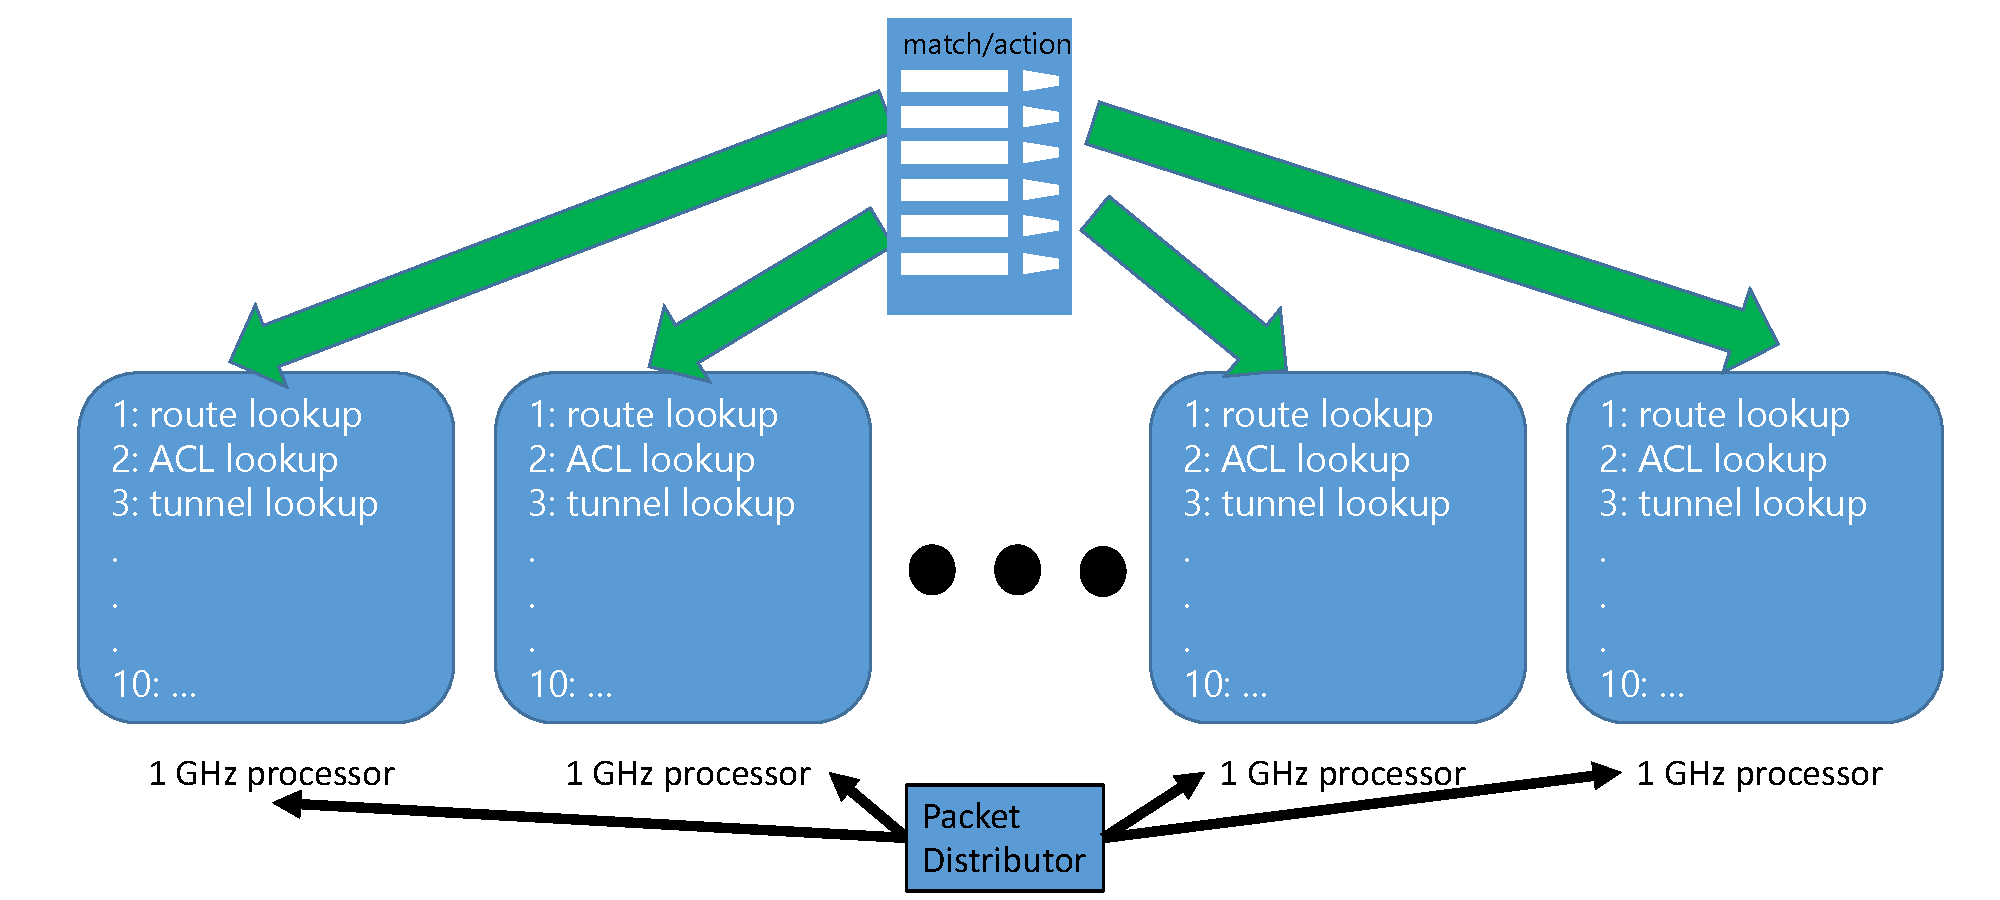
\includegraphics[width=\textwidth]{processor_array.pdf}
\caption{An array of 10 1-GHz processors. }
\label{fig:processor_array}
\end{minipage}
\caption{Two strawman designs for a high-speed router}
\end{figure}

\section{A pipeline architecture for high-speed routers}
To avoid the challenges associated with multi-ported memories, high-speed
routers are typically architected as a {\em pipeline}, where each pipeline
stage is dedicated to a fixed functionality, such as destination address
lookup, tuneling, measurement, or access control. Each pipeline stage has its
own dedicated local memory to store its own match-action tables, corresponding
to destination address lookup, tuneling, measurement, or access control, as the
case may be. This architecture provides parallelism: at any point, each
pipeline stage is working on a different packet. It also does so without
sharing memory between processors: each match-action table is local and can be
accessed only by the pipeline stage to which it belongs.

%TODO: Consider replacing "top half of ..." with a fresh figure in pptx
This pipeline architecture is the architecture followed by most high-speed
routers today. Packets arriving at a router~(top half of
Figure~\ref{domino_fig:router}) are parsed by a parser that turns
packets into header fields. These header fields are first processed by an
ingress pipeline consisting of match-action tables arranged in stages.
Processing a packet at a stage may modify its header fields, through
match-action rules, as well as some persistent state at that stage, \eg packet
counters. After the ingress pipeline, the packet is queued. Once the scheduler
dequeues the packet, it is processed by a similar egress pipeline before it is
transmitted.\footnote{In practice, the ingress and egress pipeline can be time
multiplexed on top of a single shared physical pipeline to improve utilization
of the underlying hardware~\cite{rmt}.}

\begin{figure}[!t]
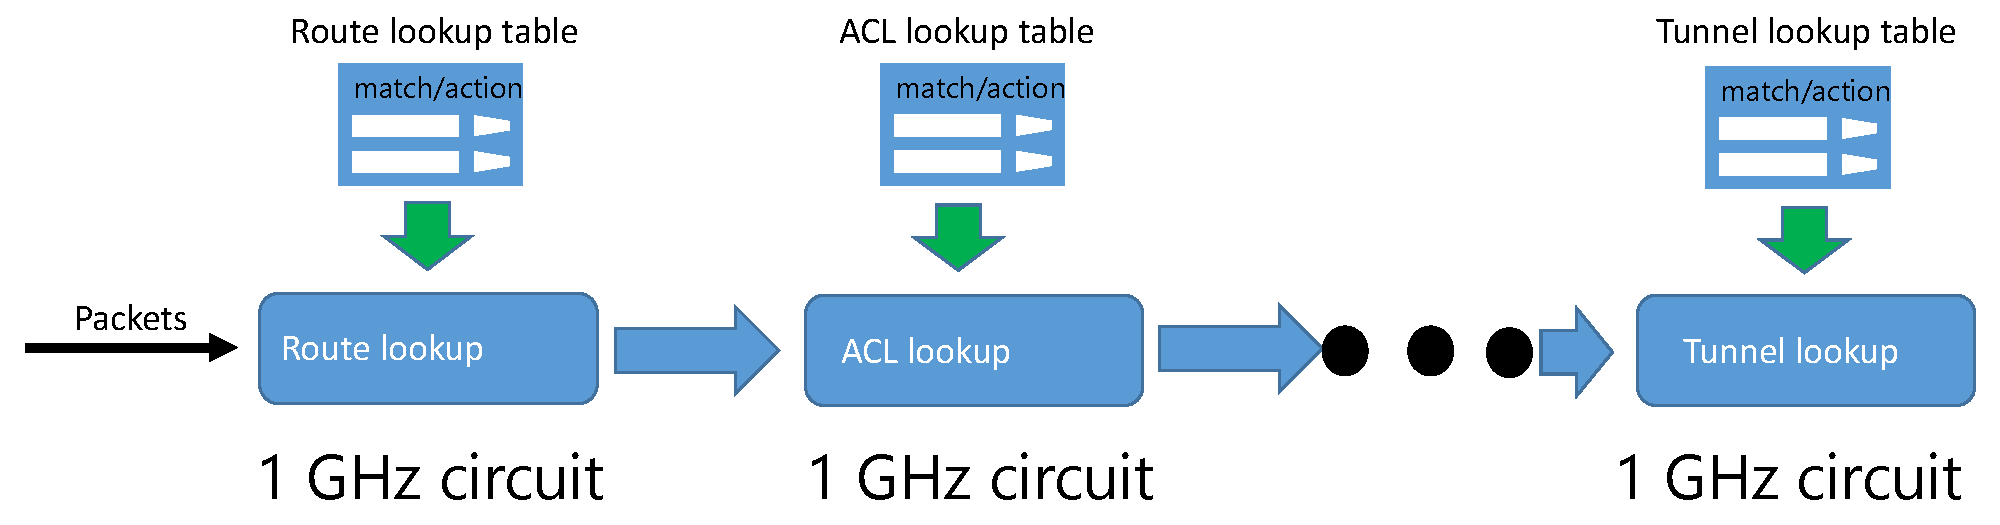
\includegraphics[width=\textwidth]{pipeline.pdf}
\caption{Pipeline architecture adopted by most high-speed routers}
\label{fig:pipeline}
\end{figure}

\subsection{The internals of a single pipeline stage} Each pipeline stage implements
the match-action model at high speed. Packets are received at a pipeline stage
at the clock rate of the pipeline's digital circuitry (\textasciitilde1 GHz).
Within a pipeline stage, the match unit extracts the relevant packet headers
from the packets so that the extracted headers can be matched against specific
patterns in a match-action table. For instance, a match unit might extract the
TCP headers out of all the packet headers to match the TCP's source port
against (say) 22 to detect SSH traffic and prioritize it as part of the action.

Once the relevant headers are extracted, they are matched against entries
stored in an on-chip match-action table. This match can either be exact (\eg
determining the next hop based on the destination's MAC address) or can use
wildcards to indicate don't-care bits in the match (\eg matching a destination
IP address against different IP subnets). The memory for the match-action table
is itself structured as a hash table (for exact matches) and a ternary
content-addressable memory (for wildcard matches).

If a match is successful, the entry that matched against the headers of the
incoming packet is returned. This entry contains the relevant information
required for the action, such as the concrete numeric value of the output port
in the case of destination-address lookup. If the packet does not match
successfully against entry in the match-action table, some default action is
carried out (such as sending the packet to the control plane CPU of the
router).

This whole process within a pipeline stage: extracting relevant headers for a
match, looking them up in a match-action table, and then carrying out the
appropriate action on a table hit or miss, can take tens of clock cycles to
finish for a given packet. At the same time, the pipeline stage must be ready
to accept a new packet every clock cycle of 1 ns. To allow this, the pipeline
stage is itself internally pipelined to allow the header extraction for one
packet to proceed in parallel with the table lookup for a second packet and the
action for a third packet.

\subsection{Flexible match-action processing}
Initially the set of fields on which matches could be performed were fixed and
limited to a small set of a standard header fields (\eg TCP, UDP, and IP).
Similarly, the actions allowed on the packet headers were restricted to a fixed
set of actions, such as dropping packet, forwarding a packet through an output
port, or setting a priority field on a packet. The common subset of match
fields and actions that were supported by most fixed-function routers was
standardized as part of the OpenFlow API~\cite{openflow}, which provided
control planes with a standardized and portable way to access the data planes
of a variety of high-speed routers.

Over time, however, the fixed nature of matches and actions led to a
progressive increase in the number of fields supported by OpenFlow~\cite{p4},
eventually leading to the development of flexible match-action processing as
embodied in recent high-speed routers~\cite{rmt, xpliant, flexpipe, tofino}. In
these architectures, a programmable parser~\cite{gibb_parsing} allows the user
to specify a new protocol format. Using this programmable parser, the router
parses bytes into this new protocol format, and the ingress and egress
pipelines can match on header fields as part of the new protocol format. This
is enabled by a input multiplexer in a match-action stage, which can extract a
user-specified field from anywhere in the packet's headers for matching. The
net result is the ability to program a router to recognize a new packet format,
then match on fields within this new format, and finally the ability to compose
new user-defined actions out of a small set of primitive actions that support
modifications to individual packet fields.

However, flexible match-action processing largely ignores the question of
flexible manipulation of {\em state} in the data plane as part of the action.
Instead, the primitive actions are restricted to {\em stateless} manipulation
of packet headers, \eg adding two packet headers and writing the result into a
third. As we will see in \S\ref{s:absmachine}, one of our contributions is
developing a machine model for programmable routers that support programmable
state modification in the data plane of the router. 

\section{Using multiple pipelines to scale to higher speeds}
Both the ingress and egress pipelines are shared across a number of router
ports.  They handle aggregate traffic belonging to all these ports, regardless
of packet sizes. When the aggregate traffic requirement is small enough, a
single ingress and egress pipleine suffices. For instance, a 64-port router
with a line rate of 10 Gbit/s per port and a minimum packet size of 64 bytes
needs to process around a billion packets per second, after accounting for
minimum inter-packet gaps~\cite{rmt}.  This requirement can be supported by a
single pipeline that runs at 1 GHz.

For higher aggregate capacities, multiple 1-GHz pipelines are required because
it is technically challenging to achieve a clock rate higher than 1 GHz in
router ASICs. While having multiple pipelines allows the router to scale to
higher aggregate speeds, it comes at the cost of fragmenting state across
different pipelines.  For instance, packets in one pipeline cannot access state
present in another pipeline, so it is challenging to maintain a piece of global
state that is accessed by and modified by every packet going through a
multi-pipeline router.

Even in a multi-pipeline router, there is a single shared piece of hardware for
the scheduler that handles inputs from multiple ingress pipelines and dequeues
its packets into multiple egress pipelines. To support the ability to handle
inputs and outputs from multiple pipelines, the scheduler's memory is
multi-ported.  This is possible without considerable area overhead by
exploiting the fact that most of the scheduler's memory is structured as a set
of first-in first-out queues with a limited set of operations (\eg enqueues and
dequeues).  

Throughout this chapter, we assume a single pipeline router for simplicity. For
concreteness, we assume the pipeline runs at 1 GHz, although our concepts
generalize to other clock frequencies as well. This is equivalent to saying
that every pipeline stage handles a new packet every clock cycle (1 ns). We
discuss multi-pipeline routers later (\S\ref{ss:multiple}). 

\section{Conclusion}
This chapter provided an overview of the hardware architecture of a high-speed
router to serve as a mental model of a router chip for the rest of this
dissertation.  The programmable hardware designs that we propose are intended
to replace fixed-function router hardware within the hardware architecture
presented here.

For instance, atoms, introduced in \S\ref{ss:intro_atoms} and detailed in
\S\ref{s:absmachine}, replace fixed action units within a match-action stage.
Our hardware design for PIFOs, introduced in \S\ref{ss:intro_pifo_hardware} and
detailed in \S\ref{s:design}, replaces the first-in first-out queues usually
found in a scheduler. Finally, the on-chip cache of our programmable key-value
store, introduced in \S\ref{ss:intro_pq_hardware} and detailed in
\S\ref{sec:aggregation}, takes the place of a match-action table within a
match-action stage. The off-chip backing store in our key-value store runs on
the control plane: either the general-purpose CPU controlling the router or a
centralized server. 
